\url{https://github.com/cedrict/fieldstone/tree/master/python_codes/fieldstone_54}

\vspace{1cm}

This stone implements three different free surface/mesh deformation algorithms. 
The first one has all the nodes move with the computed velocity (Lagrangian method)
and is coined 'method 1'. 
The second one ('method 2') only has the top row of nodes moving with the computed velocity, 
while all the nodes underneath are static (this is obviously not a viable method for 
large deformations). 
The third one ('method 3') is the method used in ASPECT and described in Rose et al (2017) \cite{robh17}.
Its implementation is described in Section~\ref{sec:freesurface}.

%...........................................................
\subsubsection*{Experiment 1 - relaxation of topography}

The domain is a 2D Cartesian box of size 512$\times$512km, with free slip on left, 
bottom and right sides, free surface at the top. 
Mantle material characterised by $\rho_m=3200$ and $\eta_m=10^{22}$. 
Gravity is vertical and Earth like. 
The surface is perturbed at startup by $\delta y = A \cos (\pi x /L_x)$ with $A$=1km.
200 time steps with $\delta t=10$kyr are carried out.
The root mean square velocity, the total volume of the domain, the min/max elevation
values of the surface are recorded over time. 

\begin{center}
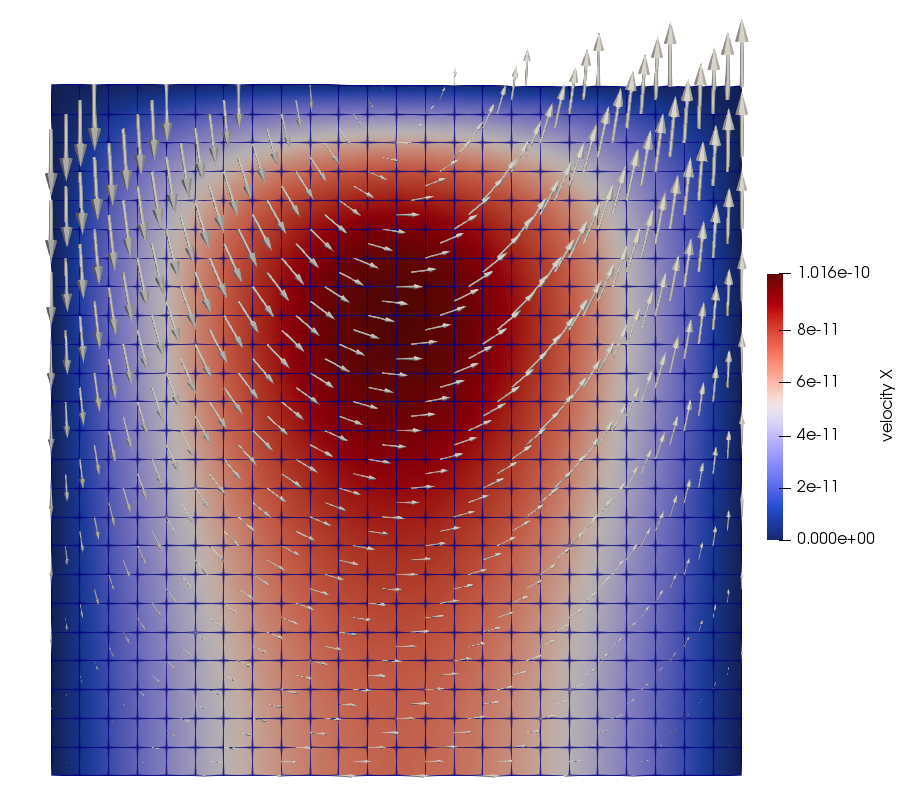
\includegraphics[width=7.5cm]{python_codes/fieldstone_54/images/exp1/u}
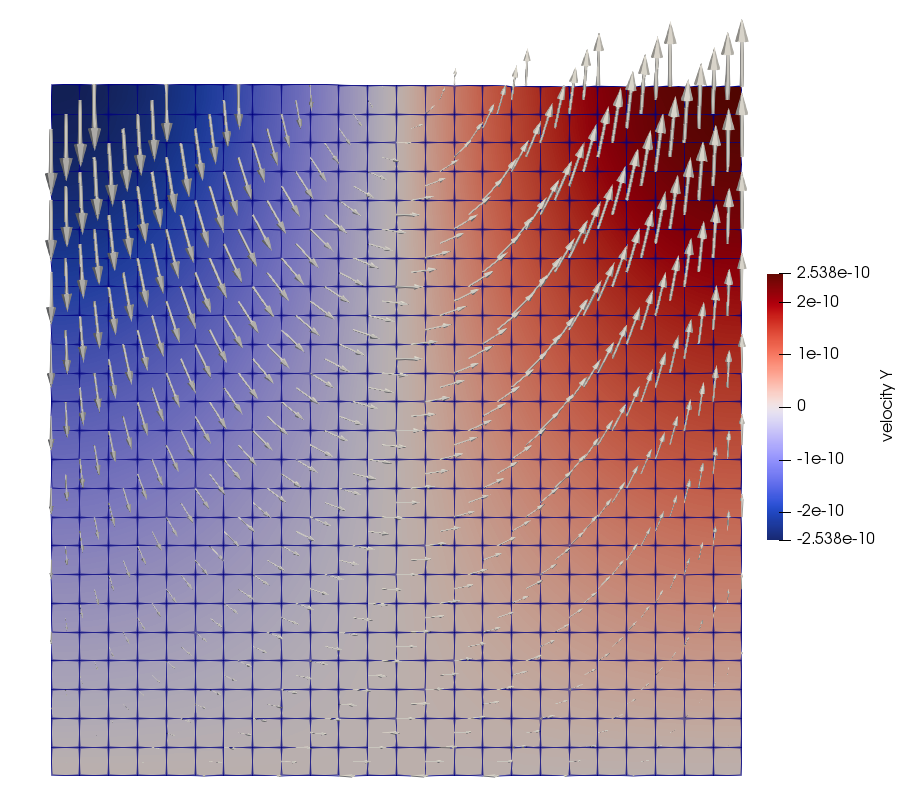
\includegraphics[width=7.5cm]{python_codes/fieldstone_54/images/exp1/v}\\
{\scriptsize velocity field at $t=0$ with resolution 24x24}
\end{center}

The results hereunder are obtained for all three methods at two different resolutions (16x16 
and 24x24 elements).
The plots on the left column are obtained with the movement of the top nodes being constrained in 
the vertical direction, while the plots on the right column are obtained with nodes being 
allowed to move in both $x$ and $y$ directions (note that for method 3 the normals are not -yet-
computed with the method of Eq. 49 in \cite{robh17} but instead by a simple geometric rule).

\begin{center}
a) 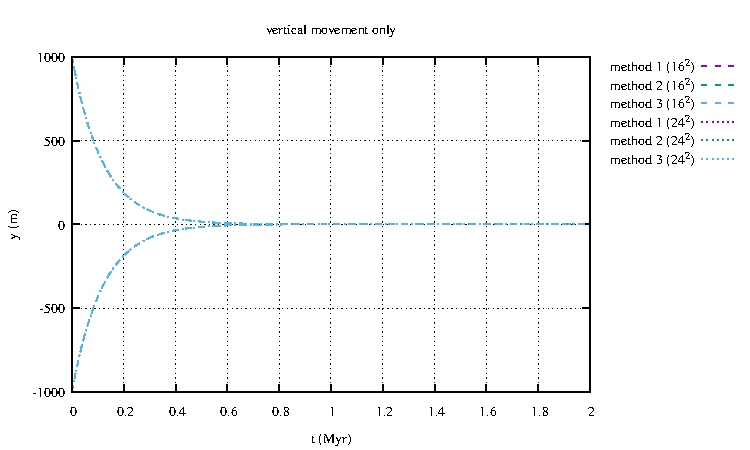
\includegraphics[width=7cm]{python_codes/fieldstone_54/images/exp1/elevation_vert.pdf}
   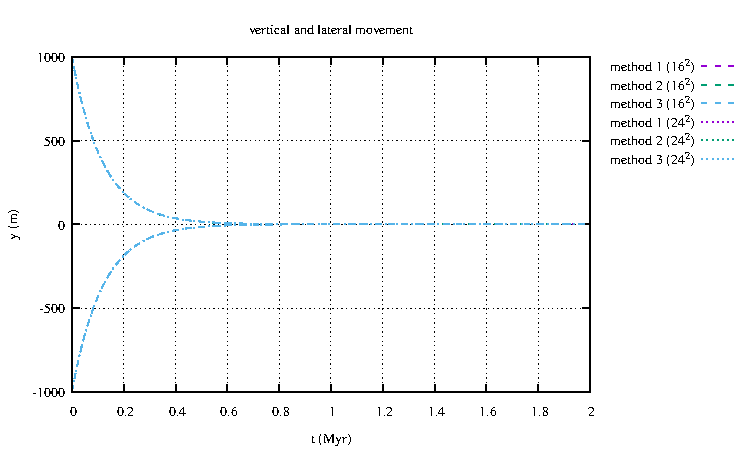
\includegraphics[width=7cm]{python_codes/fieldstone_54/images/exp1/elevation_full.pdf}\\
b) 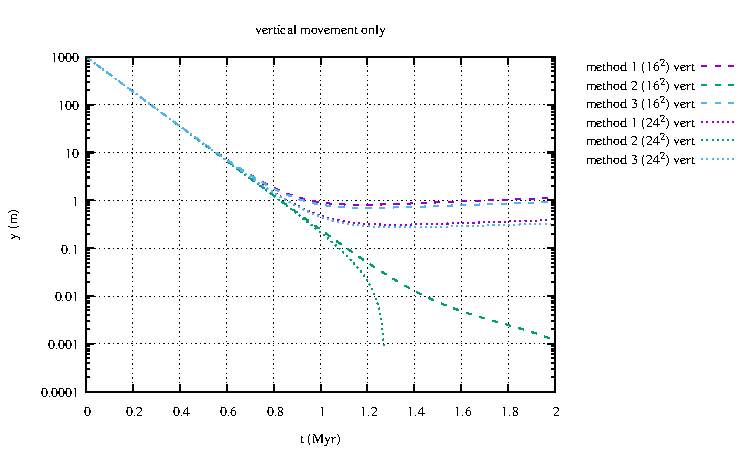
\includegraphics[width=7cm]{python_codes/fieldstone_54/images/exp1/elevation_log_vert.pdf}
   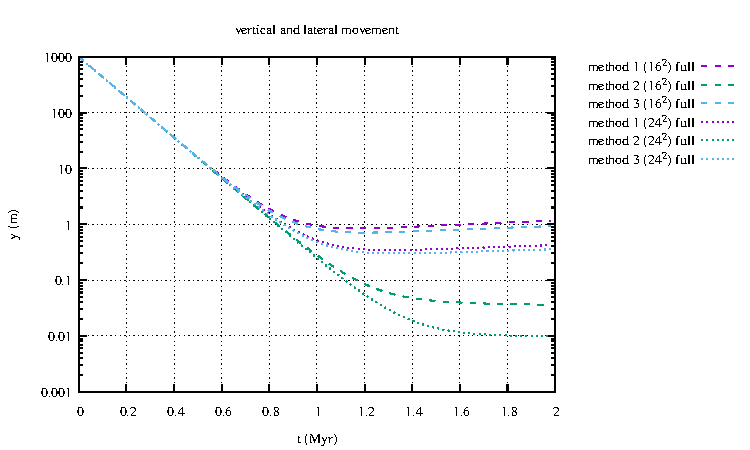
\includegraphics[width=7cm]{python_codes/fieldstone_54/images/exp1/elevation_log_full.pdf}\\
c) 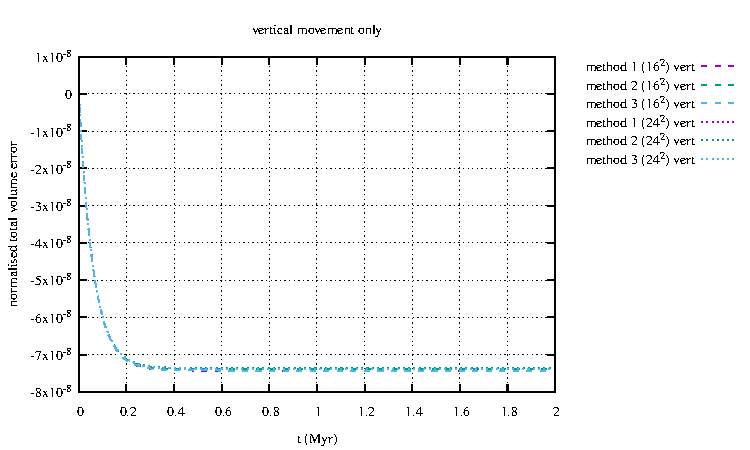
\includegraphics[width=7cm]{python_codes/fieldstone_54/images/exp1/volume_vert.pdf}
   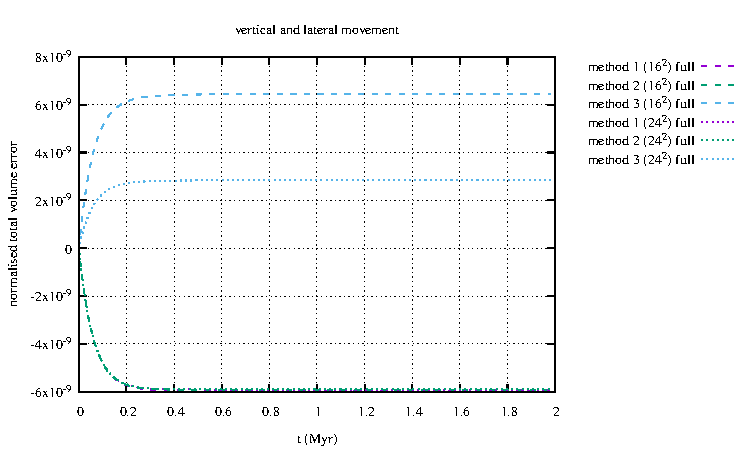
\includegraphics[width=7cm]{python_codes/fieldstone_54/images/exp1/volume_full.pdf}\\
d) 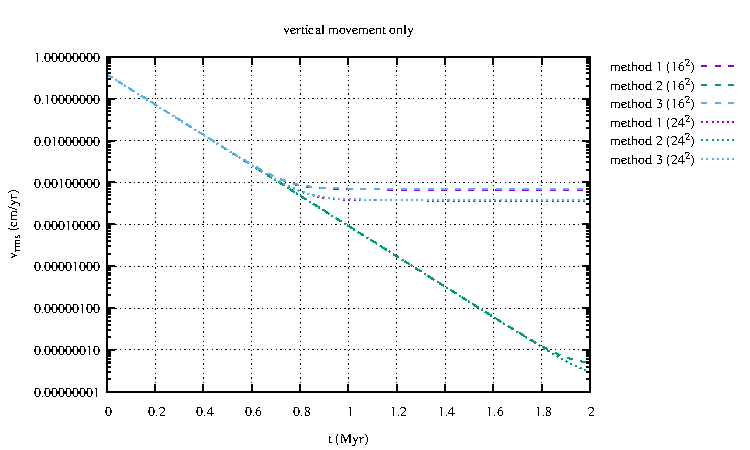
\includegraphics[width=7cm]{python_codes/fieldstone_54/images/exp1/vrms_vert.pdf}
   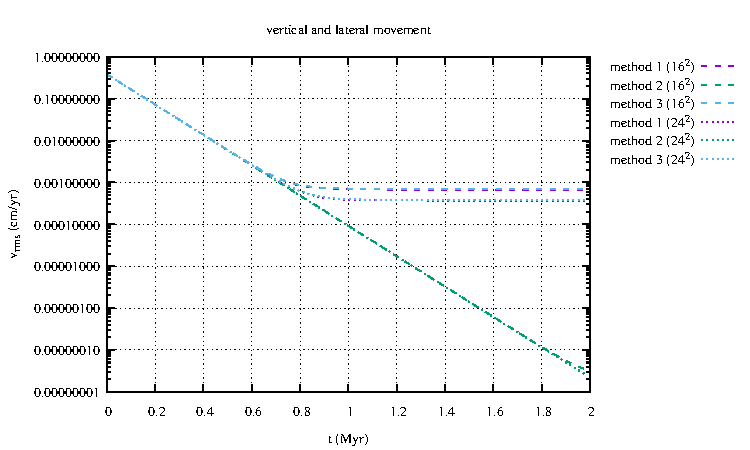
\includegraphics[width=7cm]{python_codes/fieldstone_54/images/exp1/vrms_full.pdf}\\
e) 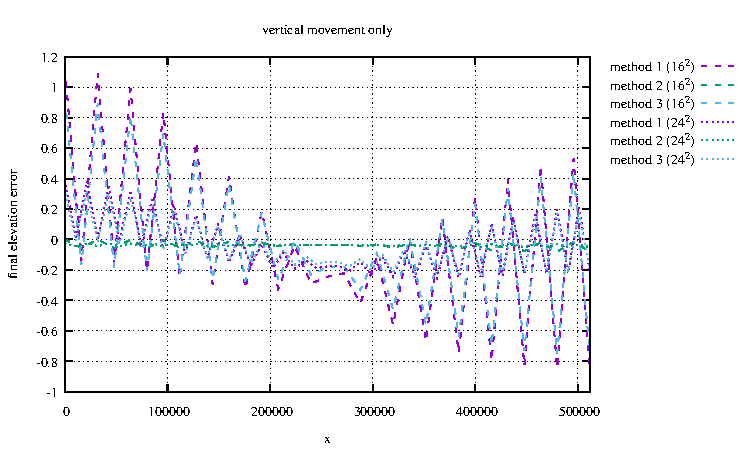
\includegraphics[width=7cm]{python_codes/fieldstone_54/images/exp1/surface_topography_200_vert.pdf}
   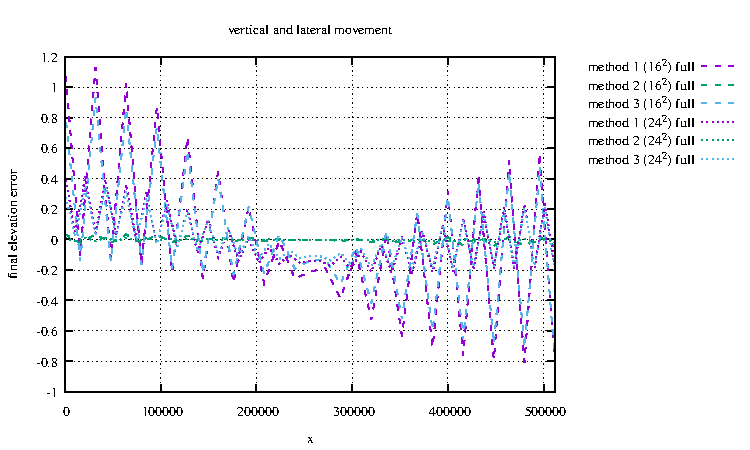
\includegraphics[width=7cm]{python_codes/fieldstone_54/images/exp1/surface_topography_200_full.pdf}\\
{\scriptsize 
a) min/max of free surface topo as a function of time; 
b) free surface topo maximum (in log scale) as a function of time; 
c) measured volume of the domain with numerical quadrature normalised by the expected volume $L_xL_y$;
d) root mean square velocity as a function of time;
e) final elevation at the 200th time step.}
\end{center}

%...........................................................
\subsubsection*{Experiment 2,3 - extension}

We now consider a rectangular domain (crust sized) of $128\times32$km, discretised by means of $40\times10$ elements.
The fluid is identical to the one above and so is gravity. 
Extensional boundary conditions are applied. In the first case, a 1cm/yr horizontal velocity is applied on both sides, while in the second case a 2cm/yr velocity is applied on the right while 0 is prescribed to the left. Free slip conditions are otherwise prescribed on the sides and bottom. 100 time steps are carried out with $\delta t=10^4$yr. Only method 3 is used here.

\begin{center}
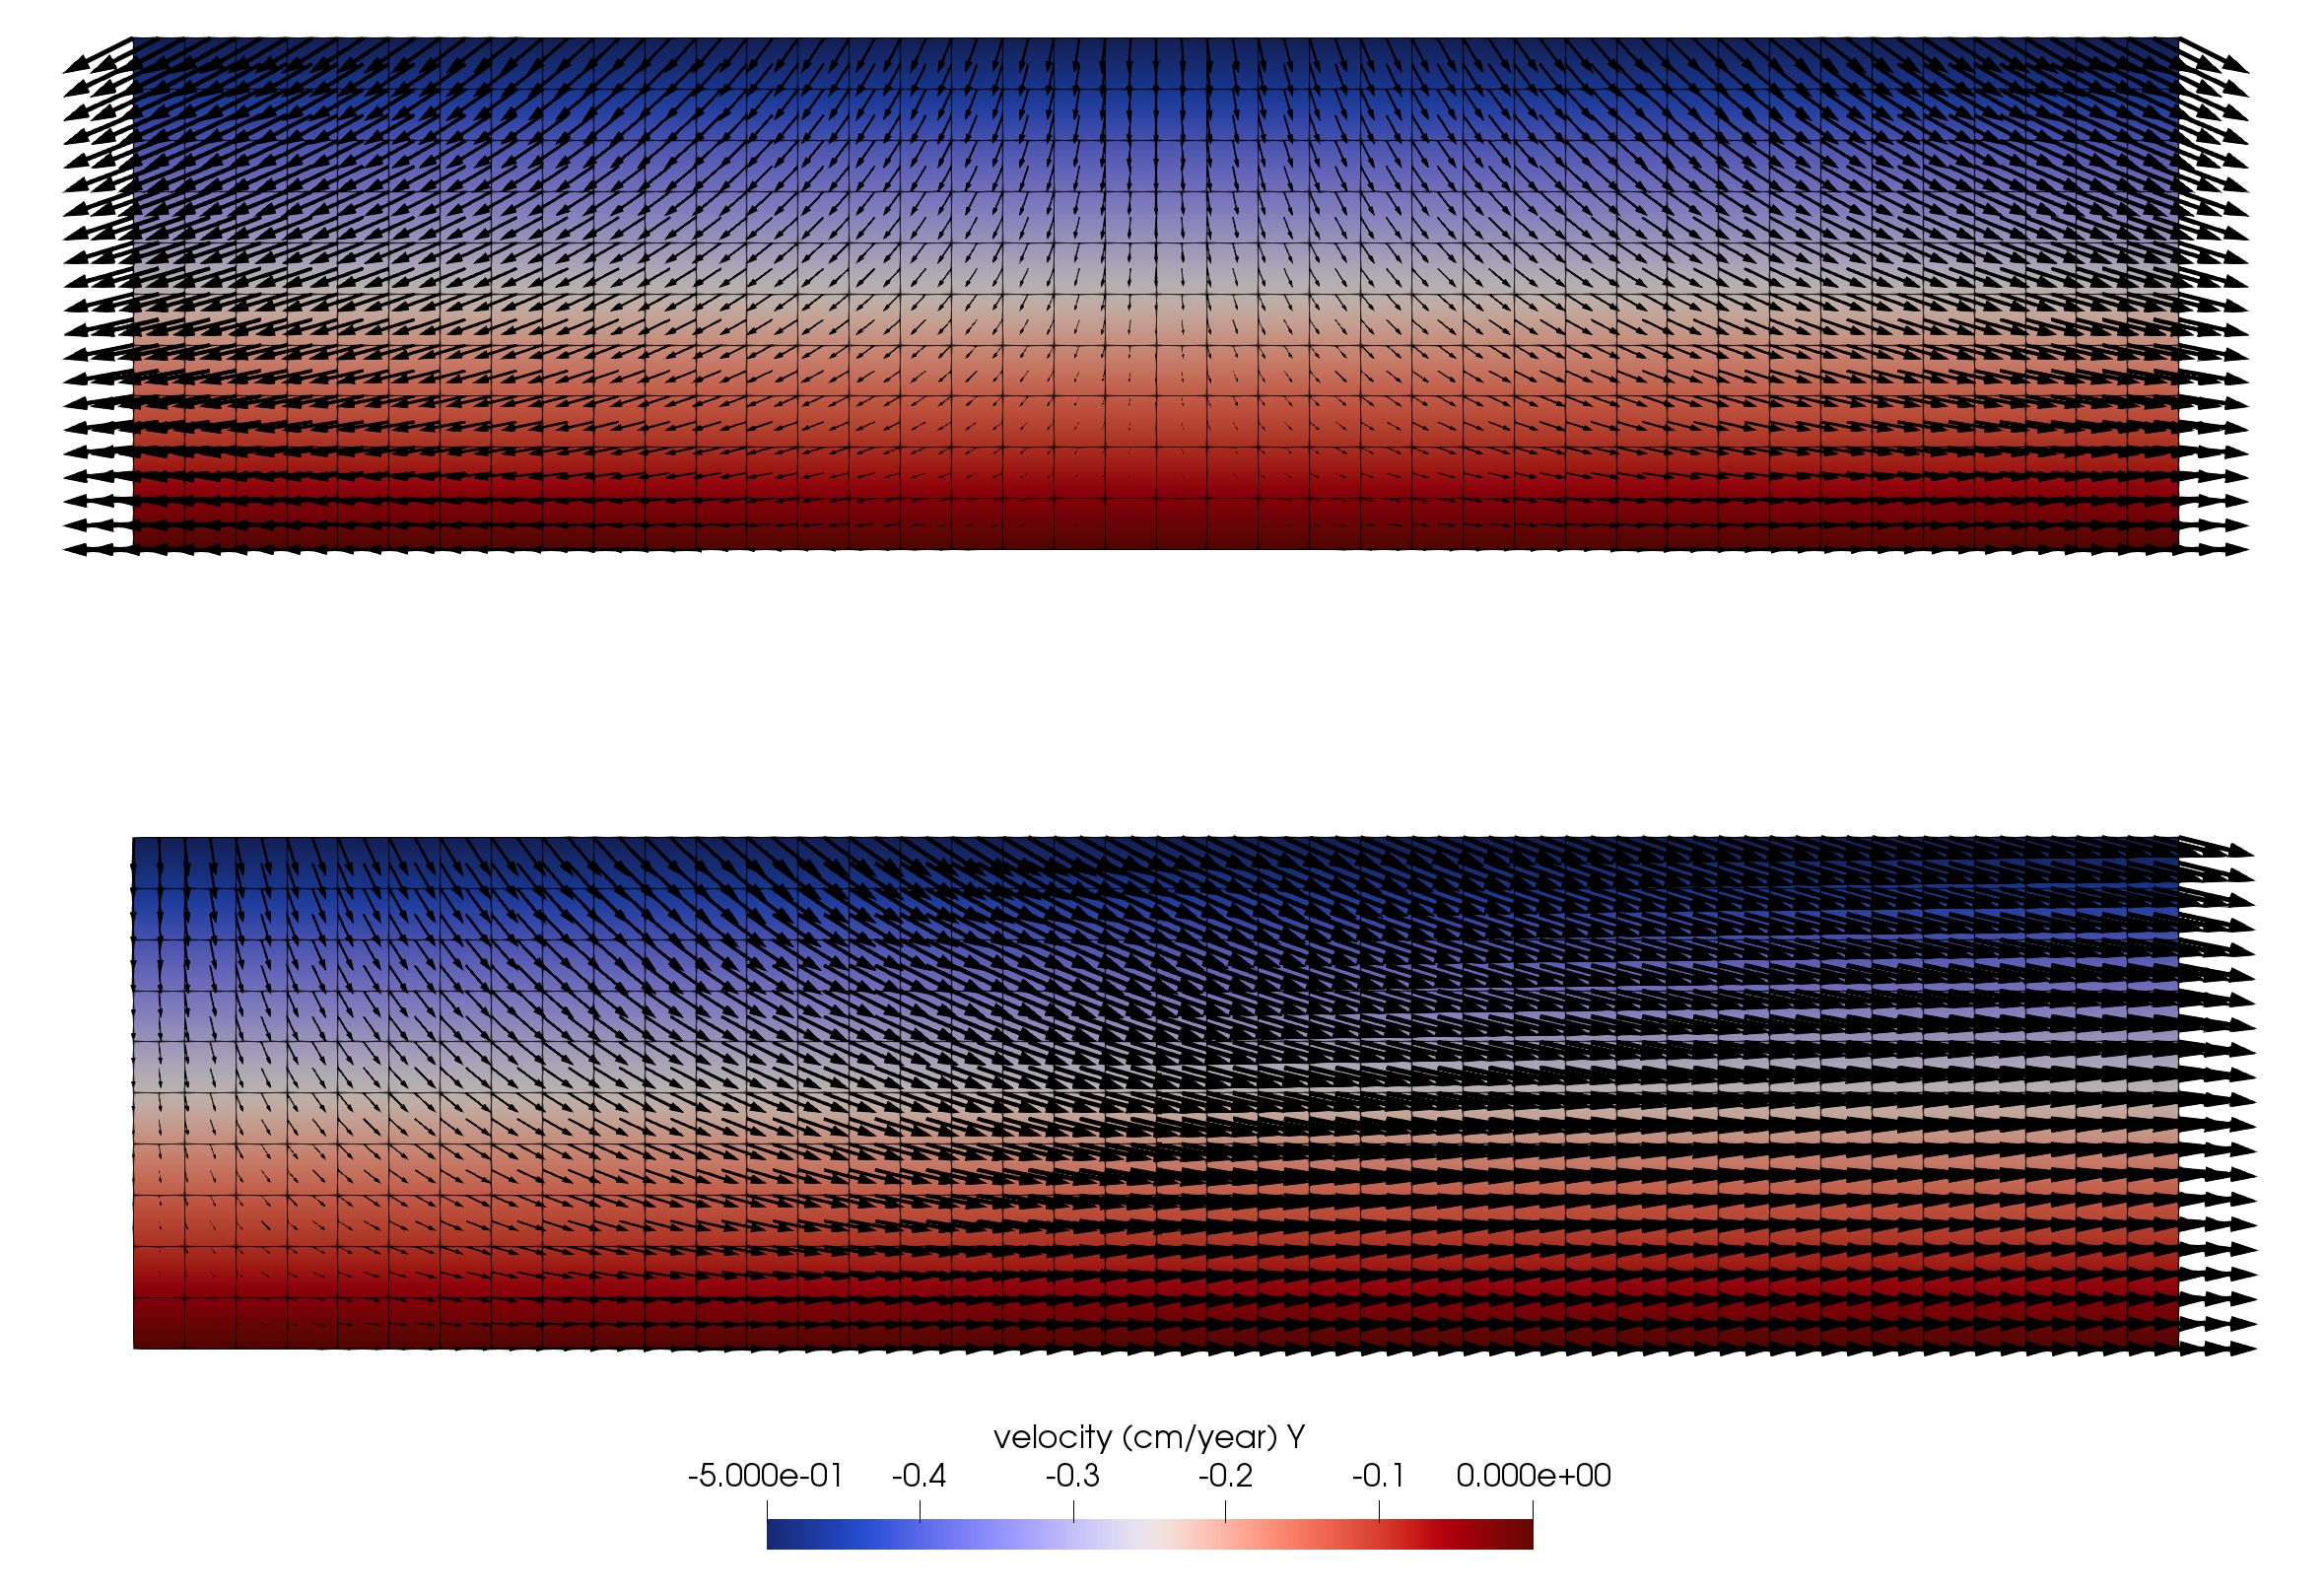
\includegraphics[width=13cm]{python_codes/fieldstone_54/images/exp2-3/vel0}\\
{\scriptsize Velocity field for both experiments at $t=0$.}
\end{center}


Despite the asymmetry in the boundary conditions, we expect the same evolution of the domain geometry. This is indeed what we recover with surprising accuracy. 'vert' stands for only vertical movement allowed (i.e. $n_x=0$, 
$n_y=1$) while 'both dir' stands for the use of dynamically computed normal vectors (based on geometrical consideration).

\begin{center}
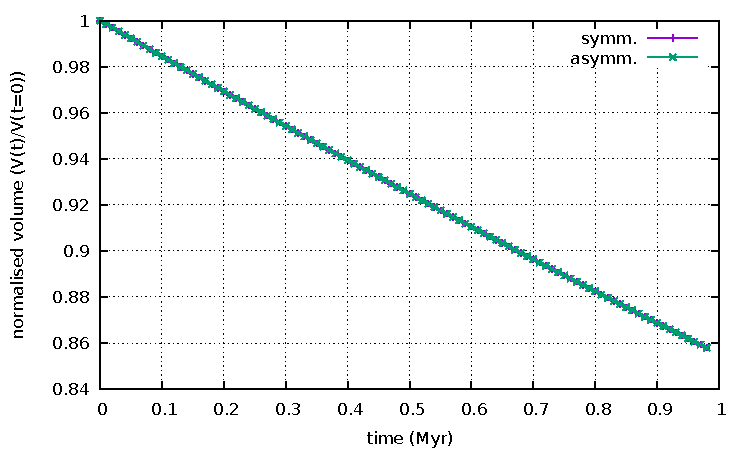
\includegraphics[width=7cm]{python_codes/fieldstone_54/images/exp2-3/volume.pdf}
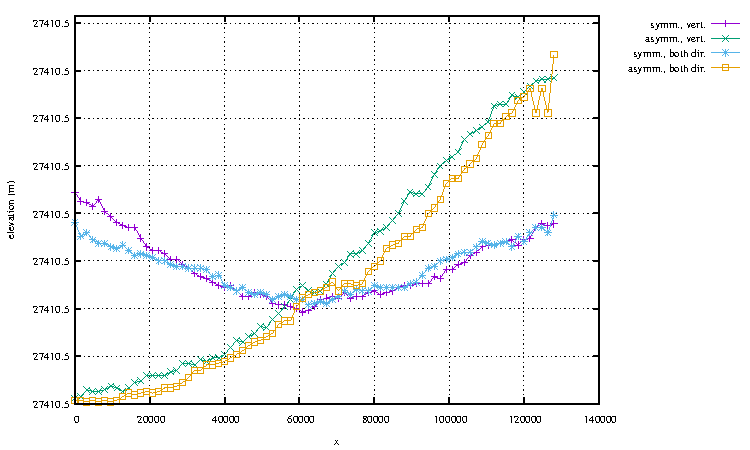
\includegraphics[width=7cm]{python_codes/fieldstone_54/images/exp2-3/surface.pdf}\\
{\scriptsize Left: time evolution of the normalised volume for both boundary condition types; Right: surface at the end of the simulation.}
\end{center}


\begin{center}
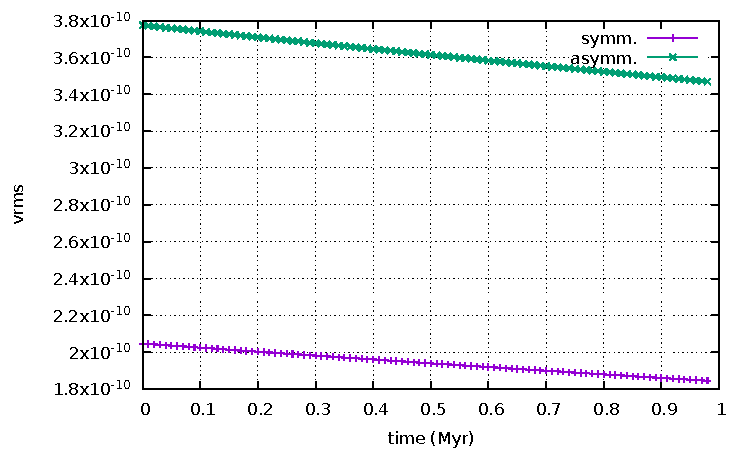
\includegraphics[width=7cm]{python_codes/fieldstone_54/images/exp2-3/vrms.pdf}
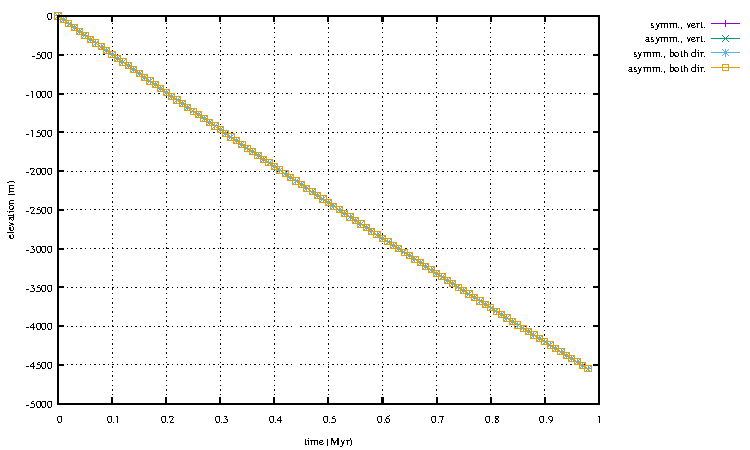
\includegraphics[width=7cm]{python_codes/fieldstone_54/images/exp2-3/elevation.pdf}\\
{\scriptsize Left: Root mean square velocity as a function of time; Right: time evolution of the elevation (min and max virtually indistinguishable).} 
\end{center}


%...........................................................
\subsubsection*{Experiment 4,5 - extension with bottom inflow}

This is the same setup as above, but we now impose an influx boundary condition at the bottom: $v=0.5cm$ (this balances the outflux exactly) and 
the horizontal component at the bottom is set to the left value (-1 or 0 cm/yr) for $x\leq L_x/2$ and to the right value +1 or +2 cm/yr for $x\geq L_x/2$.

\begin{center}
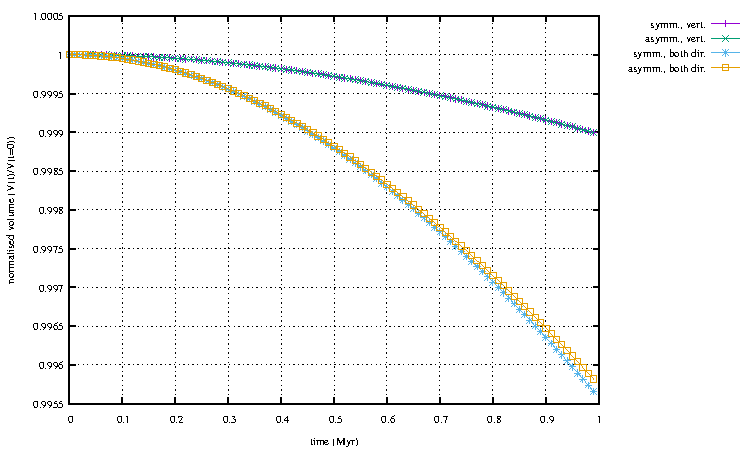
\includegraphics[width=7cm]{python_codes/fieldstone_54/images/exp4-5/volume.pdf}
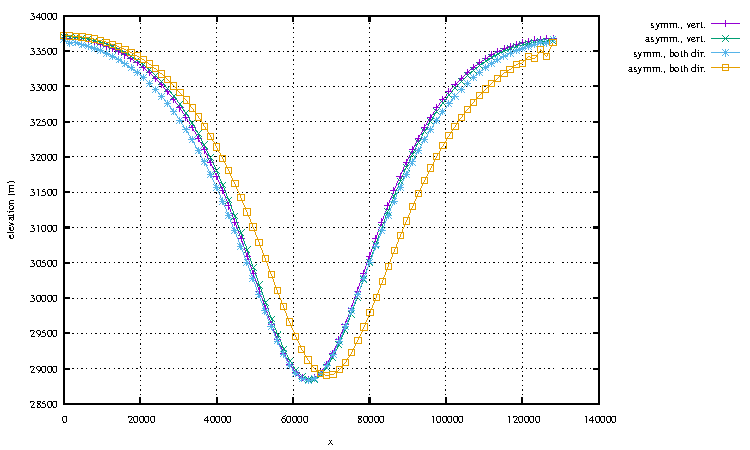
\includegraphics[width=7cm]{python_codes/fieldstone_54/images/exp4-5/surface.pdf}\\
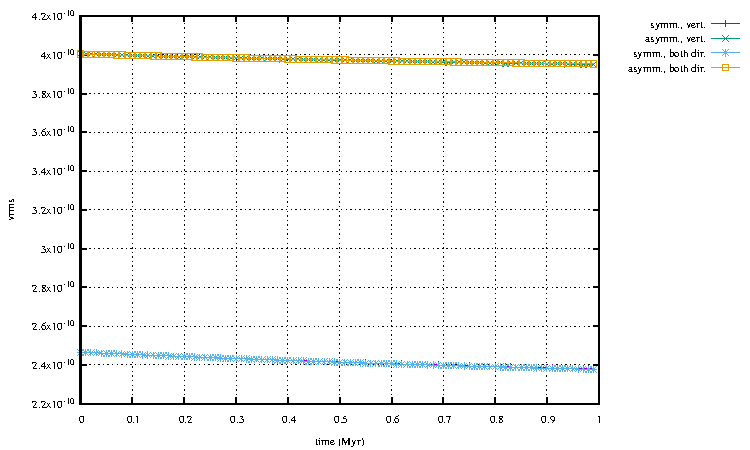
\includegraphics[width=7cm]{python_codes/fieldstone_54/images/exp4-5/vrms.pdf}
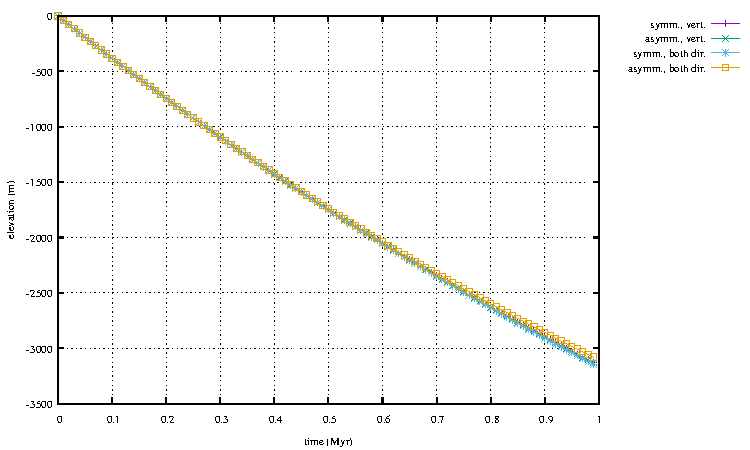
\includegraphics[width=7cm]{python_codes/fieldstone_54/images/exp4-5/elevation.pdf}\\
\end{center}

We can conclude that the 'vertical movement only' conserves volume/mass better and the free surface remains symmetrical unless the full normal is used which is simply explained by having $\vec{v}\cdot\vec{n}$ as a boundary condition: in the asymmetric extension case, the velocity is always to the right while the normal has an $x$ component which is negative and positive, therefore introducing an asymmetry in the surface boundary conditions.

\begin{center}
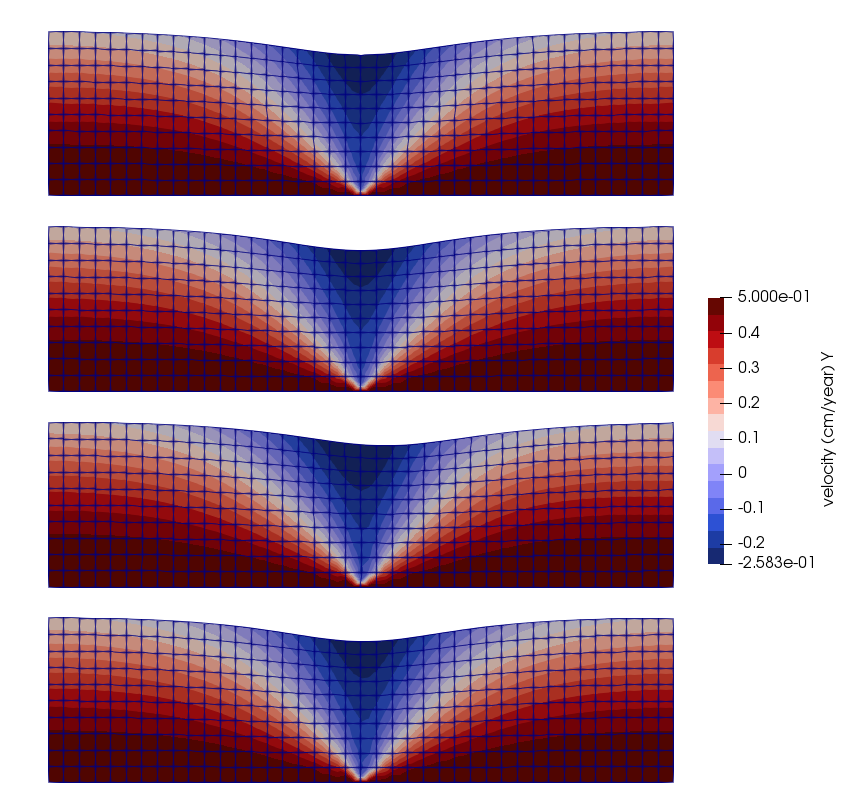
\includegraphics[width=8cm]{python_codes/fieldstone_54/images/exp4-5/v}\\
{\scriptsize Top to bottom: 
symmetric extension, full normal vector; 
symmetric extension, vertical normal vector; 
asymmetric extension, full normal vector; 
asymmetric extension, vertical normal vector}
\end{center}
%...........................................................


